\begin{frame}{The Swarm at the Edge of the Cloud}
  \vspace{1em}
  \begin{columns}
    \column{0.5\textwidth}
    \begin{figure}
      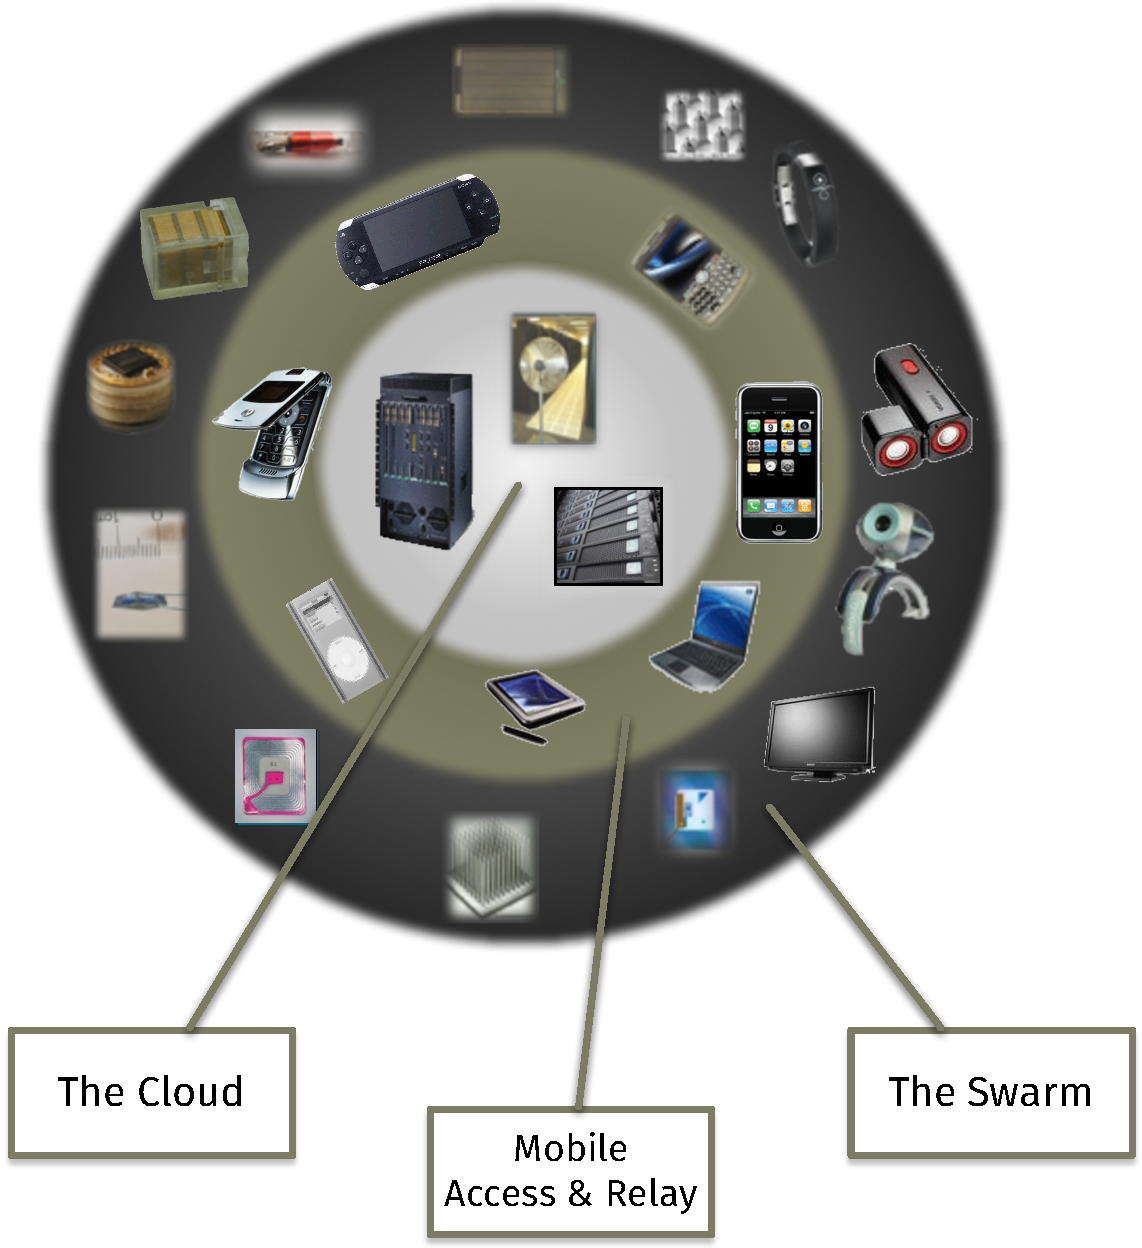
\includegraphics[width=0.8\textwidth]{figures/swarm_jan.pdf}
      \caption{J.\,Rabaey, ASPDAC'08}
    \end{figure}

    \pause

    \column{0.5\textwidth}
    Swarm, or
    \begin{itemize}
    \item \alert<4>{Internet of Things (IoT)}
    \item Internet of Everything (IoE)
    \item Industry 4.0
    \item The Industrial Internet
    \item TSensors (Trillion Sensors)
    \item Machine to Machine (M2M)
    \item Smarter Planet
    \end{itemize}

  \end{columns}
  \pause
  \begin{figure}
    
\includegraphics[width=\textwidth]{figures/swarmlogo.pdf}
  \end{figure}
\end{frame}

\begin{frame}{Gartner Hype Cycle (2015)}
  \begin{figure}
    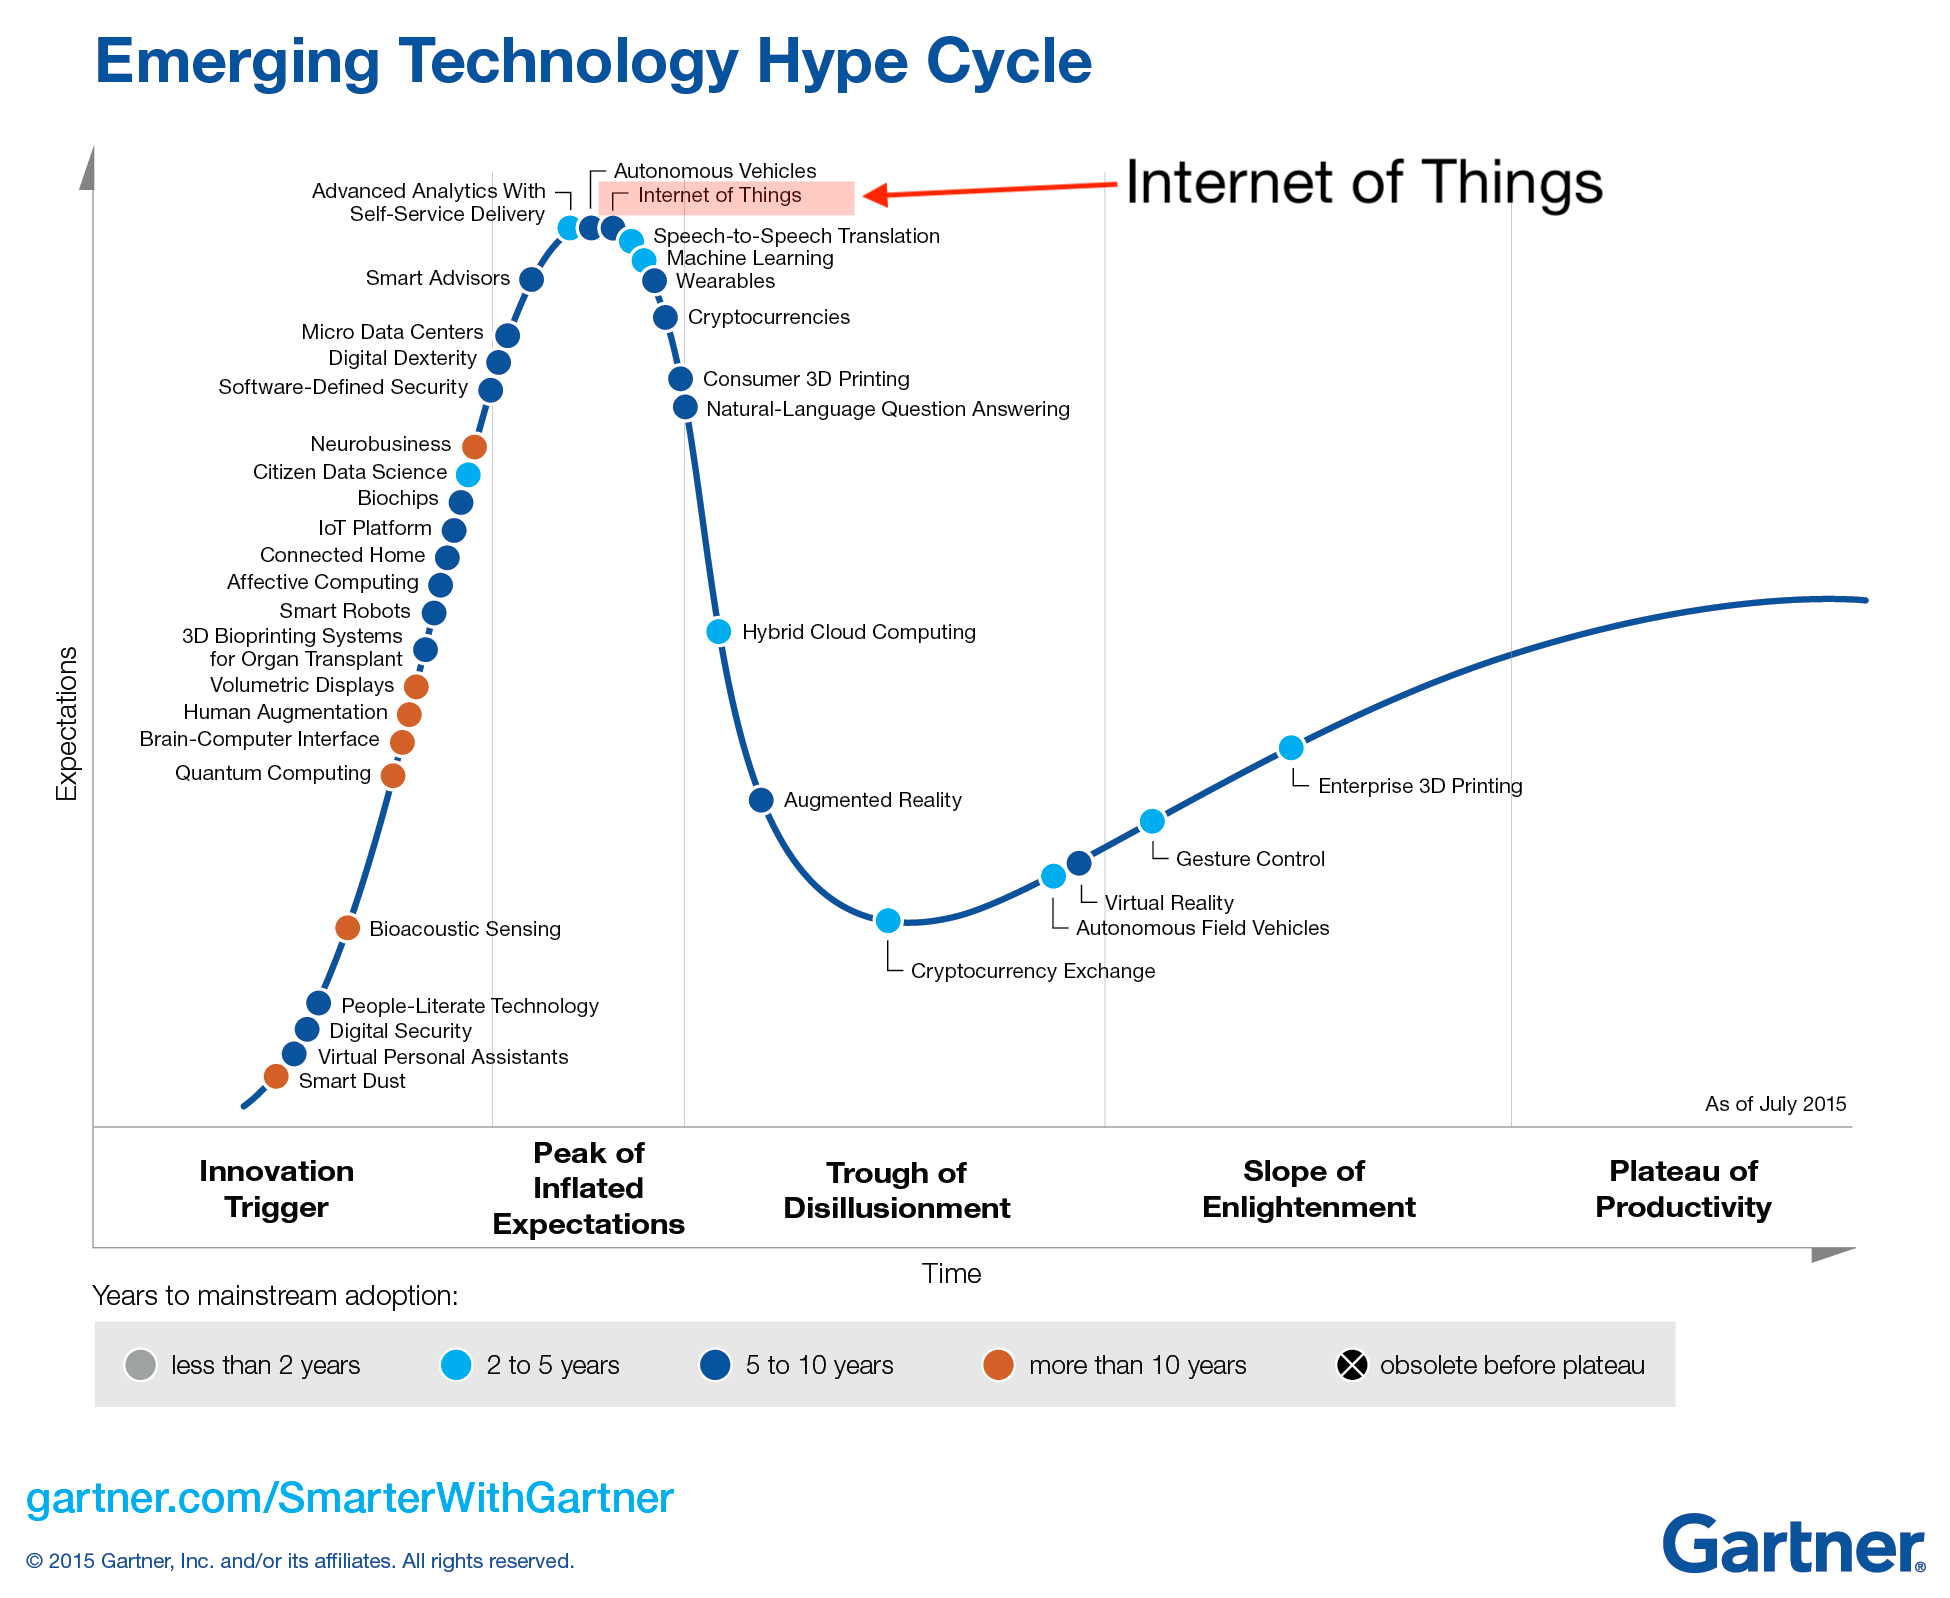
\includegraphics[width=0.8\textwidth]{figures/hype.png}
  \end{figure}
\end{frame}

\begin{frame}{A Cloud-centric Approach}
  \vspace{1em}
  \begin{figure}
    \centering
    \begin{subfigure}[t]{0.48\textwidth}
      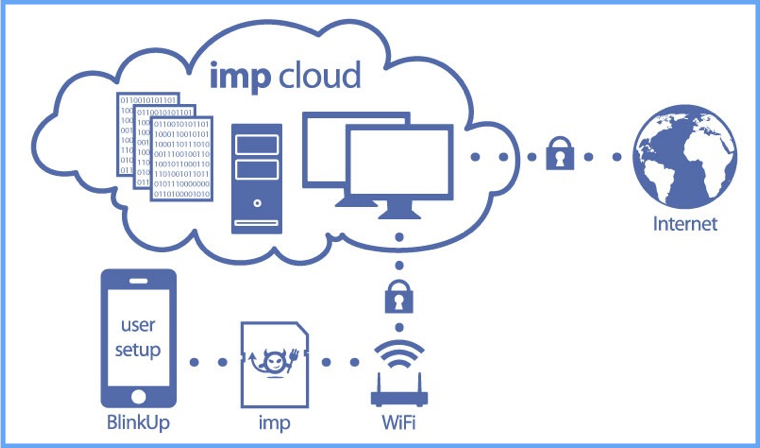
\includegraphics[width=\textwidth]{figures/cloud1.png}
      \caption{\href{http://www.limetrace.co.uk/electric-imp-platform}{Electric
          Imp}}
    \end{subfigure}
    \hfill
    \begin{subfigure}[t]{0.48\textwidth}
      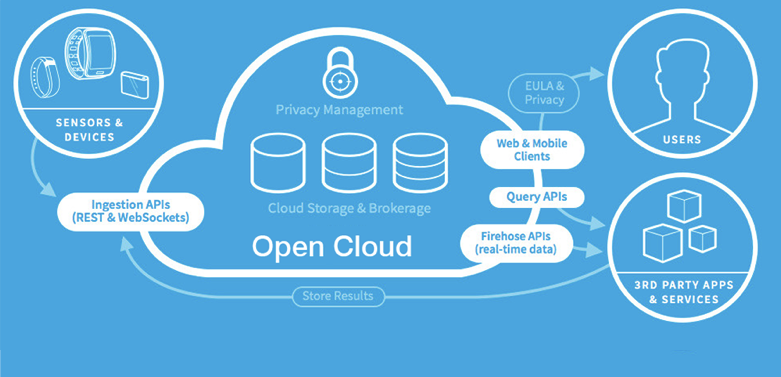
\includegraphics[width=\textwidth]{figures/cloud2.png}
      \caption{\href{https://developer.samsungsami.io/sami/sami-documentation/}{Samsung
          SAMI}}
    \end{subfigure}
    \begin{subfigure}[t]{0.7\textwidth}
      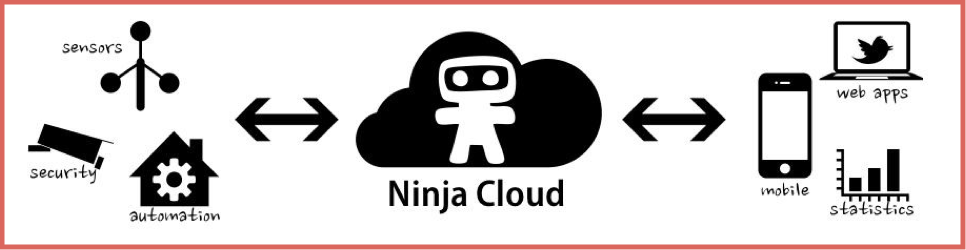
\includegraphics[width=\textwidth]{figures/cloud3.png}
      \caption{\href{http://lucept.files.wordpress.com/2012/06/ninja-blocks-capture.jpg}{Ninja Sphere}}
    \end{subfigure}
  \end{figure}
\end{frame}

\begin{frame}{``The Cloud'': Model vs.\,Reality}
  \begin{figure}
    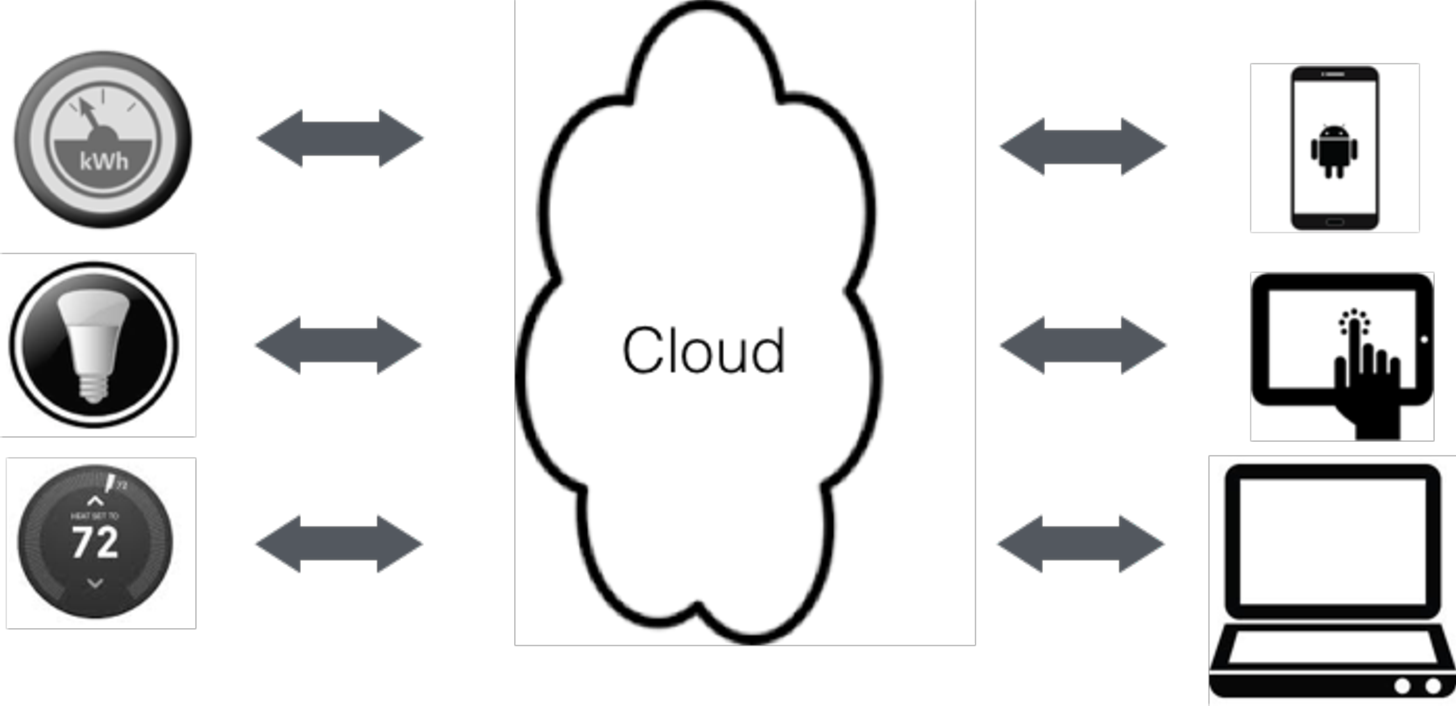
\includegraphics[width=0.6\textwidth]{figures/cloud-view.pdf}
  \end{figure}
  \vspace{-3em}
  \pause
  \begin{figure}
    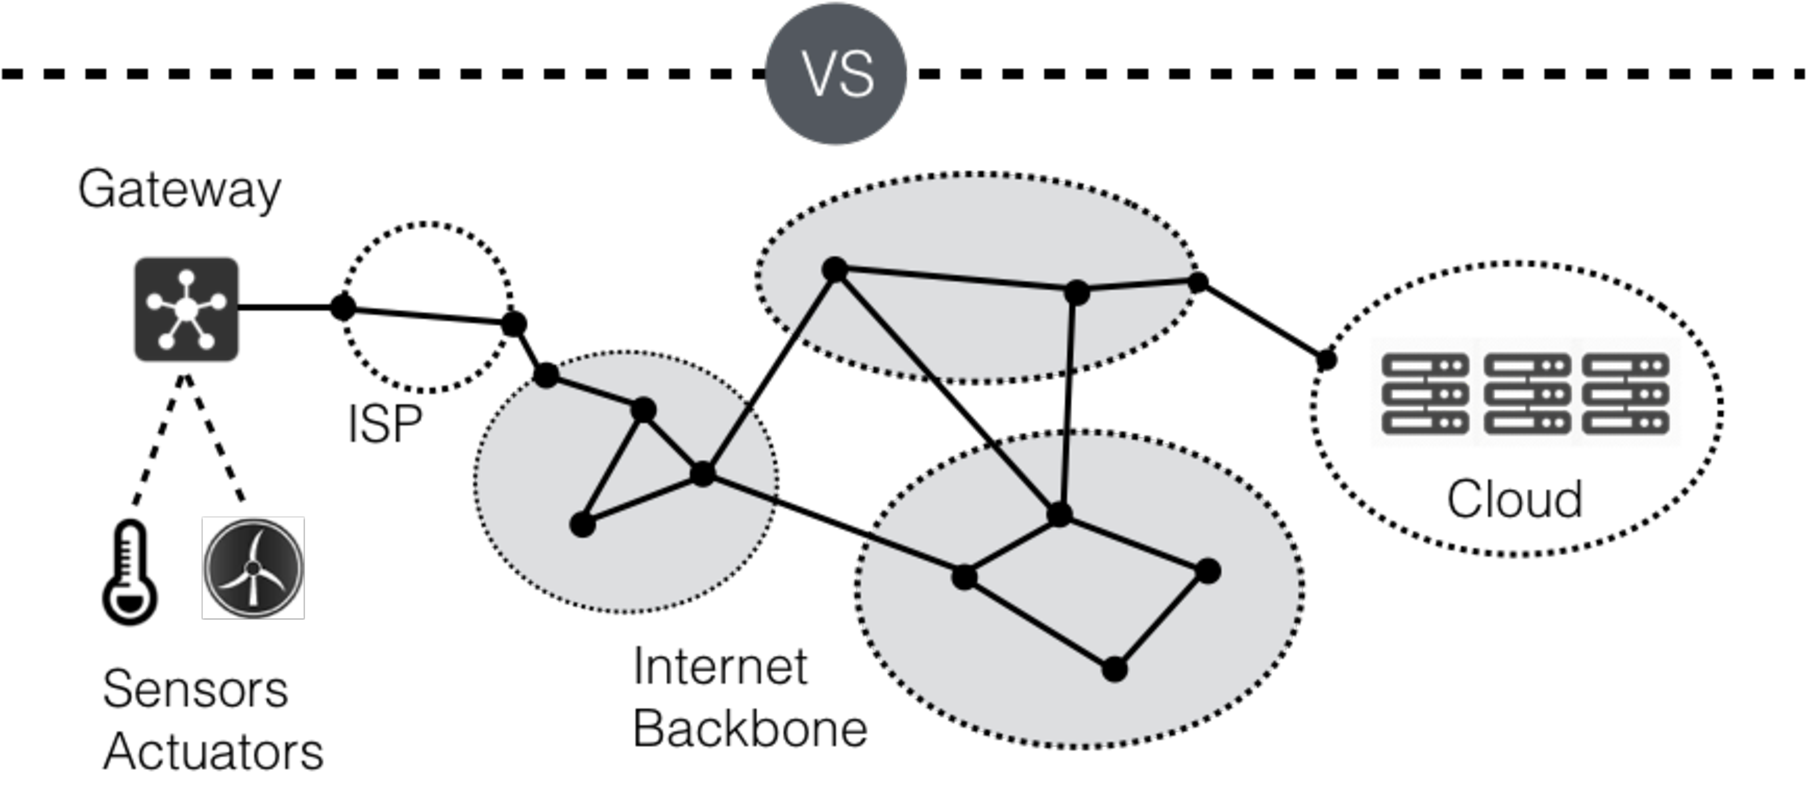
\includegraphics[width=0.7\textwidth]{figures/cloud-reality.pdf}
  \end{figure}
\end{frame}

\begin{frame}{The Cloud is Not Enough}
  \only<1>{
    \begin{table}
      \centering
      \begin{tabular}{c c c}
        \toprule
        & Web/IT & Swarm/IoT \\
        \midrule
        Privacy \& Security & Open for access & Sensitive data \\
        Scalability & Power law & Billion devices \\
        Interaction Model & Human & Machine \\
        Latency & Variable & Bounded  \\
        Bandwidth & Downstream & Upstream   \\
        Availability (QoS) & No guarantee & Requirement  \\
        Durability Management & Cloud controls & Users control \\
        \bottomrule
      \end{tabular}
      \caption{Pitfalls with Today’s Approach to IoT~\cite{zhang2015cloud}}
    \end{table}
  }
  \only<2>{
    \begin{table}
      \centering
      \begin{tabular}{c c c}
        \toprule
        & Web/IT & Swarm/IoT \\
        \midrule
        Privacy \& Security & Open for access & Sensitive data \\
        Scalability & Power law & Billion devices \\
        Interaction Model & Human & Machine \\
        \rowcolor{blue!30} Latency & Variable & Bounded  \\
        \rowcolor{blue!30} Bandwidth & Downstream & Upstream   \\
        Availability (QoS) & No guarantee & Requirement  \\
        Durability Management & Cloud controls & Users control \\
        \bottomrule
      \end{tabular}
      \caption{Pitfalls with Today’s Approach to IoT~\cite{zhang2015cloud}}
    \end{table}
  }
\end{frame}

\begin{frame}{Bandwidth}
  \vspace{1em}
  \begin{figure}
    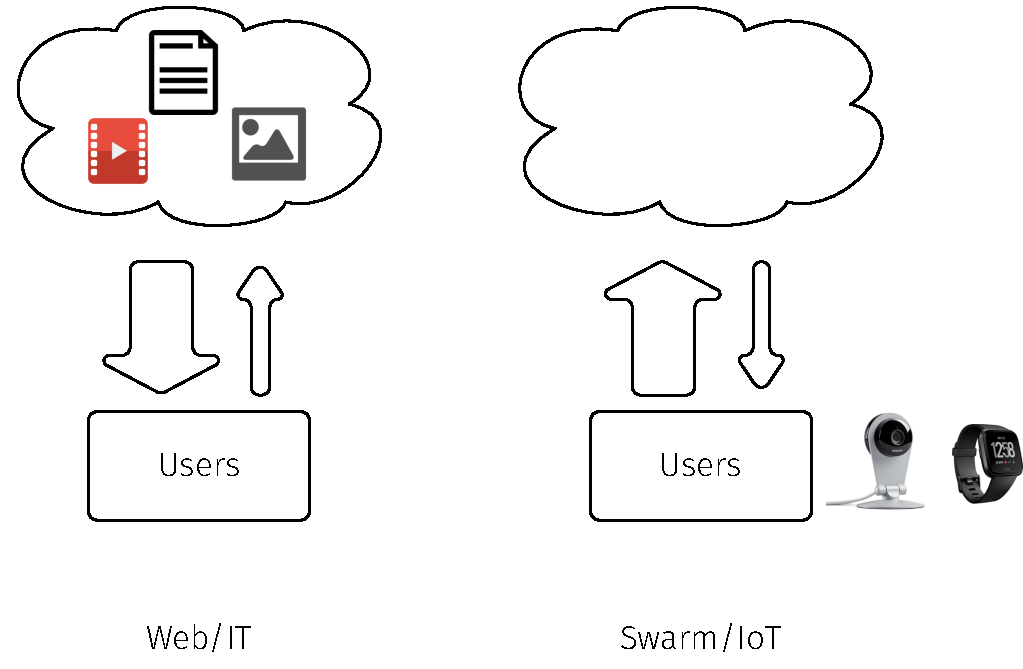
\includegraphics[width=0.9\textwidth]{figures/uplink-downlink.pdf}
  \end{figure}
\end{frame}

%%% Local Variables:
%%% mode: latex
%%% TeX-engine: xetex
%%% TeX-master: "talk"
%%% End:
